\onehalfspacing
\section{A Working Definition of Flow}
In comparison to its conceptual counterpart ``the beat'', a ``flow'' resists a clear definition in
academic and technical discourse. While there seems to be some agreement that the beat is comprised
of musically-distinct layers looping throughout a piece, definitions of flow range from anywhere as
specific as ``simply the rhythms and rhymes [a hip-hop song] contains''\footnote{
    \autocite[63]{pauledwardsHowRapArt2009}. While Edwards' statement comes within the context of an
    instruction on rapping (and therefore his reductiveness may be pedagogically useful), this attitude
    toward flow is implied by music academics who transcribe flow primarily on one line of staff notation;
    such transcriptions implicitly show flow as something existing within a fixed (or indiscernible) pitch
    space, with unambiguous, highly discernible rhythms.} 
to as wide-ranging as ``all of the rhythmical and articulative features of an emcee's delivery of 
the lyrics.''\footnote{
    \cite{kyleadamsMetricalTechniquesFlow2009}.} 
Before I name and discuss a few of the stylistic hallmarks of flow in underground hip-hop, it will be
worthwhile for me to construct a definition that ascertains what musical elements comprise it.

Consider, once more, Open Mike Eagle's characterization of his own relationship to MF DOOM's flow:
that Eagle has to be careful with it because of how much time he has spent `in DOOM's mind.'\footnote{
    \cite{estellecaswellRappingDeconstructedBest2016}. For my earlier discussion of this passage and its
    relationship to meditative listening, see Section~\ref{listeningasmeditation}.} 
The fact that Eagle can characterize his relationship to the style of DOOM's flow demonstrates that
flow encompasses more than rhythm and rhyme alone; by themselves these elements do not account for flow
as being tied to an emcee's specific or generic style. Flow, then, should be conceived more broadly than
the manifestation of rhythms through the vocal delivery of rhymes.

At the same time, however, emcees frequently describe flow as text in relation to the music, drawing
contrasts with the non-musically bounded epithet ``poetry.'' The emcee Rakim's oft-cited definition
of rap (that it is ``rhythm and poetry'') creates a distinction between texts that can be rapped and
those that are conceived within the poetic medium. Clarifying this distinction, the emcee Myka 9 of
Freestyle Fellowship offers, ``sometimes I might write a poem, a spoken-word poem, but then morph
that into a rap rhythmically.''\footnote{
    \autocite[63]{pauledwardsHowRapArt2009}.}
Myka 9's insight helps to construct a continuum for rapped text: it exists on a spectrum from
texts that are spoken in musically-bounded ways and non-musically-bounded ways.\footnote{
    Interestingly, rapped verses can be and often are delivered on varying degrees of this
    spectrum. Mitchell Ohriner notes two distinct modes of delivery, which he calls speech-rhythmic
    and music-rhythmic, based on the degree of non-alignment between the musical meter and the 
    degree to which syllable onsets correspond to metrical positions (see 
    \cite{mitchellohrinerLyricRhythmNonalignment2019}.}

This distinction between the construction of the rap as text and its performance as music is
foundational to the method by which I interrogate the concept of flow in this chapter. I believe
the techniques underground emcees employ when rapping can be neatly divided and then analyzed based
on this division, into categories I refer to as \emph{structural} and \emph{performance} techniques.
Structural techniques deal primarily with rap as text, considering its syntactic elements with primacy
over their manifestation as a stream in the musical object. By contrast, performance techniques deal
primarily with rap as music, considering the ways in which an emcee makes manifest the structures
they contrive when composing texts. Moreover, performance techniques encapsulate the decisions made
when treating the voice as an object within a digital recording. With these distinct categories,
I aim to examine how, as Mitchell Ohriner claims, flow ``encompasses phrasing, rhythm, meter, accent,
patterning, and groove, not to mention the relations among these parameters.''\footnote{
    \autocite[28]{mitchellohrinerFlowRhythmicVoice2019}.}

\section{Thesis Statement \& Definitions}
In this chapter, I examine a few notable techniques that underground emcees employ in structuring
and performing their flow, arguing that, like producers, their choice to use these techniques reaches
listeners as underground. The four techniques I define below do not form an exhaustive list, but rather
are salient and illustrative in how they relate to my conception of the subgenre. My terms are also 
divided into the subcategories of structural and performance techniques, a distinction I draw in my 
understanding of how emcees work with the text that makes up their flow. When the underground emcee 
inhabits the role of writer, they experiment with structuring techniques including \emph{pivot rhyme} 
and \emph{closing fragmentation} to craft their verses. Stepping into the recording booth or onto the 
stage, the emcee shifts into their role as rapper and therefore draws on performance techniques such 
as \emph{mimesis} and \emph{processing} to shape their vocal delivery. Each of these techniques serves
as the focus one of the close-readings that follow, so I will clarify their functions before I examine
repertory.

As a device for constructing a verse, a pivot rhyme allows an emcee to execute a shift in end rhyme;
it occurs when the concluding words of the previous bar conjure up an idea that is semantically linked 
to the bar's topic but does not rhyme. In this instance, the rapper chooses to displace the lyric past
the next bar line, allowing that word or phrase to serve as the primary rhyming sound within a new repetition
of the beat pattern. Often the emcee uses this instance as a way to play with audience expectation, taking
the listener's focus on this final rhyme to shift towards a topic semantically distinct from the previous bar.

Underground emcees employ closing fragmentation as another method of structuring a verse, particularly
to mark the end of some sort of formal section. To accomplish this, emcees will deliver a ``full'' textual
phrase, usually structured as a setup and punchline, then signal a close through breaking up and repeating 
the component elements of that textual phrase in a more improvisatory and loosely-organized style of delivery.
Fragmentation and repetition here do not function as they do in the construction of a hook; rather, they
demonstrate to the listener that some larger textual unit\textemdash a phrase, a verse, the song 
itself\textemdash is ending.

With both performance techniques, emcees articulate the role of their voice as a layer \emph{amongst} the rest 
of the mix, rather than the principal element within it. In particular, the use of mimesis, or stylizing vocal 
delivery to mimic other elements in the beat layer, draws attention to the other musical elements in an attempt
to foreground their musicality. This promotes the other musical layer to a co-soloist role, rather than 
functioning as a background loop or layer, allowing the listener to focus on it as more than just accompanimental
structure beneath the vocal flow.

Processing more generally refers to the manipulation of digital audio after its recorded (especially through
the use of EQ, compression, and reverb software or hardware), but here I use it to refer to methods of altering
the vocal signal as a method of electronic composition. In particular, rappers use processing effects like delay, 
distortion, and pitch transposition to alter the audio of their voice during or after tracking it to treat it 
as a musically manipulable element; the vocals here function as \emph{sound} inasmuch as they do text.\footnote{
    My definition of processing here is a broader version of the definition of ``glitch'' in Chapter 2 
    (see p.~\pageref{glitch}.)}
In this way, processing treats the voice as if it were any other musical layer and, as a result, any layer can
be listened with as much consideration as the voice.


%\newpage
\section{Structuring Techniques}
Perhaps more than any other musical element in the rap song, the transcription of flow makes clear the
limitations of staff notation. Throughout this project, my dedication to transcription in standard notation
arises from my desire to mimic what Kofi Agawu conceptualizes as a ``post colonial transcription,'' one based
in an ``ideology of sameness so that\textellipsis we can gain a better view of difference.''\footnote{
    \autocite[67]{kofiagawuInventionAfricanRhythm2003}. Agawu's chapter traces a history of non-African scholars
    transcribing Northern Ewe drumming in a way that both essentializes and exoticizes African music as primarily
    rhythmic and therefore fundamentally different from Western approaches to music making. Although I do not wish
    to employ colonization uncritically as a metaphor for music theory's relationship to hip-hop, I do believe that
    the same essentializing and exoticizing tendencies would manifest if I were to completely avoid standard notation
    for this repertory.}
However, this approach exists at odds with another point Agawu notes: no singular mode of representation can 
sufficiently convey the totality of a musical listening experience.\footnote{
    \autocite[187]{kofiagawuAfricanRhythmNorthern1995}.}
In dealing with flow as an independent, textual structure from its musical manifestation, I will opt to use
another mode of representation: namely, Ohriner's $modulo$ 16 grid transcriptions\footnote{
    For a detailed overview of the system and a few sample transcriptions, see 
    \autocite[xxviii--xl, 7--9]{mitchellohrinerFlowRhythmicVoice2019}.}

Ohriner's method of transcription simplifies certain elements that become problematic when transcribing 
flow in standard notation. First, his 16-point grid for a bar avoids proliferate use of eighth, sixteenth,
and thirty-second notes, not to mention syncopation between them. Subsequently, his method also simplifies 
the naming structure by labeling each metric position with a number from 0--15; one can more succinctly
communicate a syllable landing on ``the third sixteenth note of beat 3'' as position 10, for instance. 
Finally, Ohriner's system does not necessitate a transcriber to choose fixed metrical positions in the 
same way standard notation and adaptations of TUBS for flow do; if a syllable onset occurs slightly before
the beat, this can be accounted for simply by moving the corresponding circle. Although vocal groove and
non-alignment with the meter is not a focus in this chapter, the ability for a system to adapt between
quantized and non-quantized rhythms is foundational to being able to transcribe flow.

\phantomsection
\subsection*{\centering Madvillain's ``Great Day''}
\addcontentsline{toc}{subsection}{Madvillain's ``Great Day''}

Madvillain, the moniker under which DOOM and Madlib released all of their collaborations except for
``One Beer,'' looms large in the world of underground hip-hop. One unrelenting focus of the accolades
their 2004 double LP \textit{Madvillainy} has received is DOOM's flow: in the words of Ta-Nehisi Coates,
``[\textit{Madvillainy}'s] singular sound came mostly from [DOOM's] raspy baritone rendering a sort of
nerdcore poetry.''\footnote{
    \cite{ta-nehisicoatesMaskDoomNonconformist2009}.}

This claim to DOOM's uniqueness, eccentricity, and artistry finds purchase beyond the mythologizing in
which Coates and much of the rest of the hip-hop community partake. Kyle Adams, for instance, notes that
on ``All Caps'' both the melodic samples (various portions of the main theme for the NBC crime drama 
\textit{Ironside}) and DOOM's flow ``[seem] to float free of the meter, being only weakly tethered to
it by the drum sample.''\footnote{
    \cite{kyleadamsMetricalTechniquesFlow2009}. What Adams notes about the \textit{Ironside} sample likely
    bolsters my claim that sample slippage is a frequently employed technique in underground hip-hop production,
    but it is not uniformly employed across Madlib's sampling practice (more on this below).}
Adams arrives at this characterization of DOOM's flow in examining the structure of its syntax: particularly,
how rhymes in ``All Caps'' do not often fall in regular metrical places and that syntactical units (or phrases) 
often cross metrical boundaries. DOOM's novel use of this irregularity, per Adams, contributes to the perception
of DOOM as an alternative rap artist.

While metrical ambiguity and enjambment may play a role in DOOM's sounding as underground on ``All Caps,''
I am hesitant to accept this as the whole picture of DOOM's alternative identity. A counterexample to the
techniques Adams accounts for on ``All Caps'' emerges from the track that immediately follows it on 
\textit{Madvillainy}\textemdash ``Great Day.'' The beat's primary melodic sample comes from ``How Do You
Believe,'' an instrumental funk track by Stevie Wonder, released in 1968 under the alias Evits Rednow.
Madlib aligns the sampled elements (electric piano, harmonica, bass, and auxiliary percussion) closely
with the drum break he uses, ushering in a hypermetric downbeat with a C-sharp minor blues lick every
fourth bar in the A section.\footnote{
    This type of metric regularity also pervades ``One Beer'', where the whole instrumental before
    the skit is sampled from one track by the funk band Cortex (see Section~\ref{samplebased}.)}

Figure~\ref{fig:doomfirstpiv} shows how DOOM, as might be expected, flows with a syntactical structure
of a  similar regularity. Avoiding the downbeat where the sample loops, he raps: ``Mad plays the bass 
like the race card, / Villain on the case to break shards and leave her face scarred.'' Over these two 
bars, DOOM structures a setup and punchline within the confines of the barline, in addition to landing 
the two-syllable rhyme that closes each bar on positions 12 and 14. The internal rhyme in the second bar
(``break shards'') occurs in a metrically weaker position (6 to 8, as opposed to 4 to 6), but falls
within what Ohriner refers to as the same durational segment (in this case, a value of 2 on the grid). 
Rather than interrupt the sense of regularity in the flow, I argue the internal rhyme in this bar 
creates an anticipation for the rhythmically ``restored'' position of the end rhyme.
\clearpage

    \begin{figure}[!ht]
        \centering
        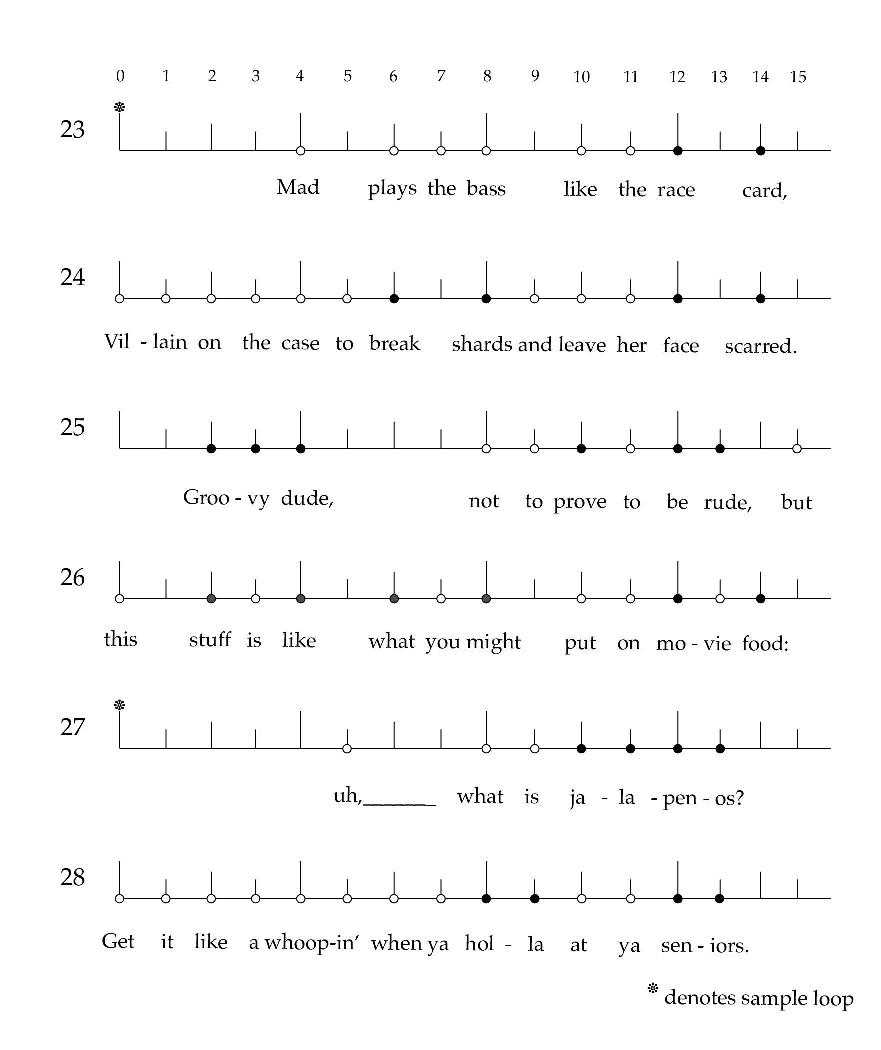
\includegraphics{images/figures/chp 03/059115greatdayfirstpivot.pdf}
        \caption{First pivot in Madvillain's ``Great Day,'' 0:59--1:15.}
        \label{fig:doomfirstpiv}
    \end{figure}

Over the next two bars, DOOM's flow becomes slightly more complex, anticipating the four bar loop
of the sample. Bars 25 and 26 increase the number of syllable onsets from 18 to 22, as well as the 
frequency, position, and syllable count of the rhymes. In the setup bar, DOOM creates an internal 
rhyme with ``Groovy dude'' and ``prove to  be rude,'' each fitting within a durational segment of 2
from positions 2--4 and 10--12, respectively. In the punchline, ``movie food'' once again restores
the metric position of the end rhyme, preceded by two softer, internal rhymes (``stuff is like'' with
``what you might'' falling between 2--4 and 6--8). Despite the increase in internal complexity, the 
syntactic structure of these bars remains normal: DOOM fits a sentence structured ``$x$, but $y$'' 
within the same time span as the previous setup and punchline.

My focus on the regular structure in the first four bars is important for establishing a connection
to the next four, two of which I transcribed as a part of Figure~\ref{fig:doomfirstpiv}. I perceive 
a semantic link in the content of bars 26 and 27 that allows DOOM to pivot to a new rhyme scheme but
in the process invites me as a listener to anticipate something different. My expectation at the end 
of  bar 26 is that DOOM is going to rap about butter: not only because I put it on ``movie food,'' 
but also because he has done so twice already on the album up to this point.\footnote{
    DOOM refers to his ``buttery flow'' on ``Raid'' and Madlib's beats as ``so butter'' on ``All 
    Caps.''}
DOOM, of course, thwarts these expectations, positing ``jalapenos'' as if it were a botched 
\textit{Jeopardy!} answer. He draws out a humorous semantic link between these two bars, drawing
me in to the word which becomes the focus of his rhyme scheme in the oncoming quatrain. With its
final two syllables falling on positions 12 and 13, jalapenos ushers in a set of highly regular
lines, each ending with ``holla at ya seniors,'' ``hashish fienda,'' and ``grass is greener''
in the same metric positions.

DOOM's first humorous pivot and the regularity of the subsequent quatrain provide crucial context
for a similar moment between bars 34 and 35, an instance where I would apply the term pivot rhyme.
Figure~\ref{fig:doomsecondpiv} overviews a quatrain with a similarly regular structure. ``Wishes'' 
falls on positions 11 and 12, displaced 1 position forward from the ends of the two following 
syntactic  closes: ``mad glitches'' and ``jaw twitches.'' The closely related structuring of the 
middle bars of the quatrain set the listener up to hear: ``One thing this party could use is more\textellipsis
booze.''And he makes that ellipsis audible! As a reviewer for \textit{Pitchfork} notes, ``the rhyme's 
pattern and rap's topical stereotype demands the word `bitches,' but [DOOM] hilariously uses `booze'
instead.''\footnote{
    Quoted in \cite{estellecaswellRappingDeconstructedBest2016}.}
Indeed, DOOM's patterning of flow, his regulating of syntactic structure, and his harnessing of
listener's expectations concerning rhyme lead into this moment; he crosses a barline, intentionally,
yet again giving the listener a moment to expect one close to the phrase, before veering off in 
another direction.

    \begin{figure}[!ht]
        \centering
        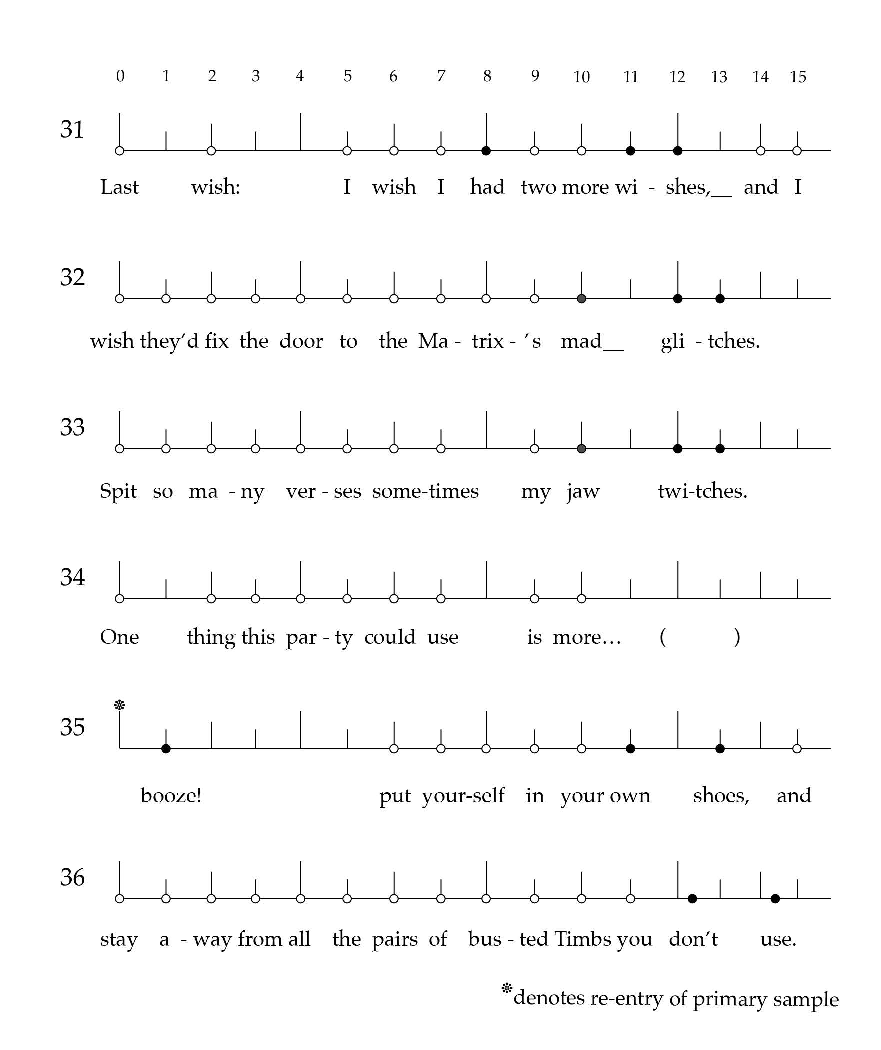
\includegraphics{images/figures/chp 03/121137greatdaysecondpivot.pdf}
        \caption{Second pivot in Madvillain's ``Great Day,'' 1:21--1:37.}
        \label{fig:doomsecondpiv}
    \end{figure}

\phantomsection
\subsection*{\centering Armand Hammer and R.A.P. Ferreira's ``Dead Cars''}
\addcontentsline{toc}{subsection}{Armand Hammer and R.A.P. Ferreira's ``Dead Cars''}

\begin{itemize}
    \item Armand Hammer (billy woods and ELUCID) is a recent premiere (?) underground hip-hop duo out of
    New York, the flagship artist for Backwoodz Studioz
    \item \textit{Shrines} (2019) was a follow up to their critically-acclaimed \textit{Paraffin} (2018) 
    and ``Dead Cars'' a point of exchange with the Ruby Yacht collective; it features R.A.P. Ferreira 
    (owner-operator of the label) and Kenny Segal (a frequent collaborator with both the Ruby Yacht and 
    Backwoodz Studioz roster).
    \item ``Dead Cars'' features a series of short verse-sections from all three artists: at 64 bpm, 
    the three are ``trading 8s''\textemdash  ELUCID begins, woods follows, ELUCID returns, then Ferreira's
    feature enters
    \item Ferreira's verse is marked by a drastic shift in the musical texture: the drums drop out, a
    new Rhodes EP melody is layered in, and reversed audio samples are used to recomposed the chord
    loop
    \item The transcription Figure~\ref{fig:roryclosingfrag} picks up in the early mid-verse, 
    two bars prior to the drum's re-entry
        \begin{itemize}
            \item Ferreira's verse, although slightly varied in the placement of syllables throughout,
            remains consistent in it's placement of rhyming syllables slightly in anticipation of positions
            4 and 12; in lieu of snare drum hits, these orient us within the instrumental texture
            \item As the drums re-enter, Ferreira delivers only two syntactic units (``Bronze Kafka
            metamorph, Black Orpheus set the course / in the Backwoodz, jiggin' with no remorse'') throughout
            the second half of his verse part.
            \item This technique functions as a kind of signposting; we know once Ferreira begins
            fragmenting and repeating text that the verse (or verse-part, in this case) is drawing
            to a close. I call this \textit{closing fragmentation}
        \end{itemize}
    \item This technique resembles the two of Duinker's definitions: hook-sections are typified by
    lyrical repetition and fragmentation, and looser-organized vocal sections comprised of ``ad-hoc,
    ametric vocals, skits, or\textellipsis [rapping] that doesn't function like a verse or hook.''
        \begin{itemize}
            \item Duinker's categorizations make some helpful distinctions, but Ferreira's closing
            fragmentation technique avoids a clear fit in one section or the other. 
            \item The lyrics are fragmented/repeated, but Ferreira situates them within the verse's
            rhyme scheme and patterning of the vocals.
            \item Their content be characterized as the type of ``hype'' vocals Duinker identifies
            (Ferreira is doing is due dilligence by shouting out Backwoodz as a collective, much
            like a hype vocalist shouts out producers involved with the making of a track), but
            the vocals are still presented as if they are a verse-part, not something appended to
            the end of a track.
            \item Closing fragmentation, then, becomes a valuable way to describe an emcee's use
            of fragementation and repetition within the context of verse, if the emcee uses those
            tools to create a ``tag'' like ending.
        \end{itemize}
    \item As a listener, I've encountered closing fragmentation most prominently in Ferreira's 
    discography, but the tool is not idiosyncratic to his approach. On ``Dead Cars,'' both ELUCID
    woods employ it to a lesser extent at the close of their verse-parts. Additionally, other members
    of the Ruby Yacht collective, especially Pink Navel and S.AL, have picked up on the technique.
\end{itemize}

    \begin{figure}[!htp]
        \centering
        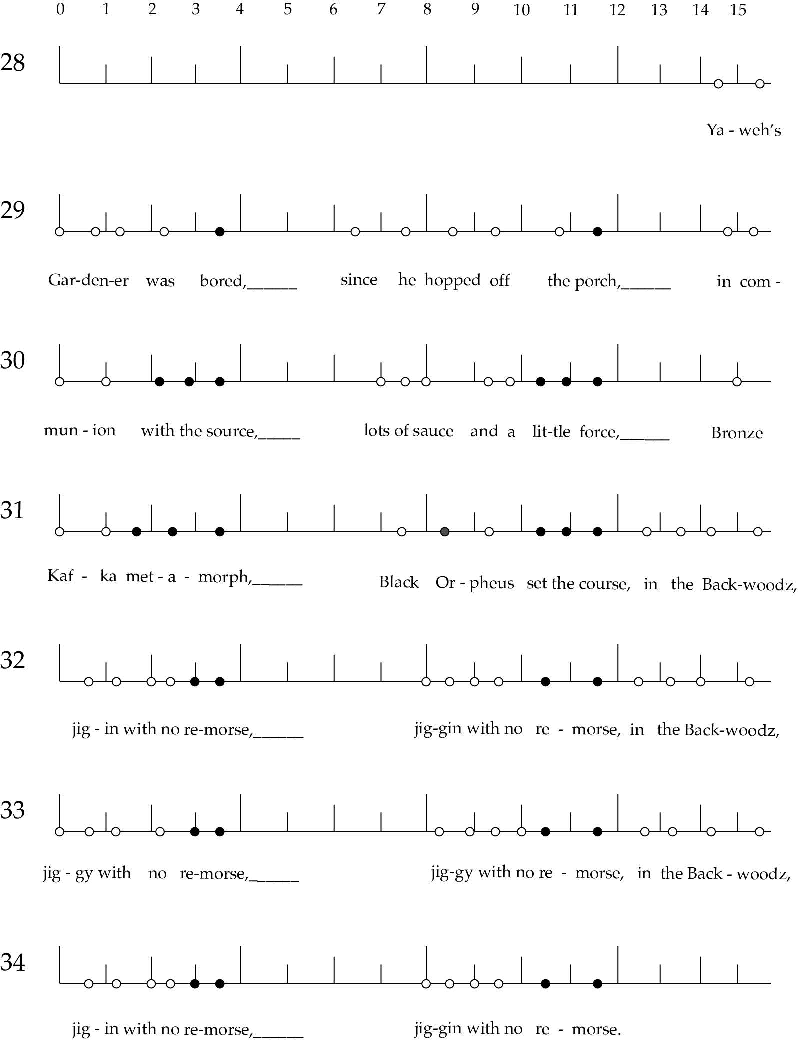
\includegraphics{images/figures/chp 03/144206deadcarsendfrag.pdf}
        .\caption{Closing fragmentation in ``R.A.P. Ferreira's ``Dead Cars,'' 1:44--2:06.}
        \label{fig:roryclosingfrag}
    \end{figure}


\newpage
\section{Performance Techniques}
\phantomsection
\subsection*{\centering R.A.P. Ferreira -- ``NONCIPHER''}
\addcontentsline{toc}{subsection}{R.A.P. Ferreira's ``NONCIPHER''}
    
    \begin{figure}[!htp]
        \centering
        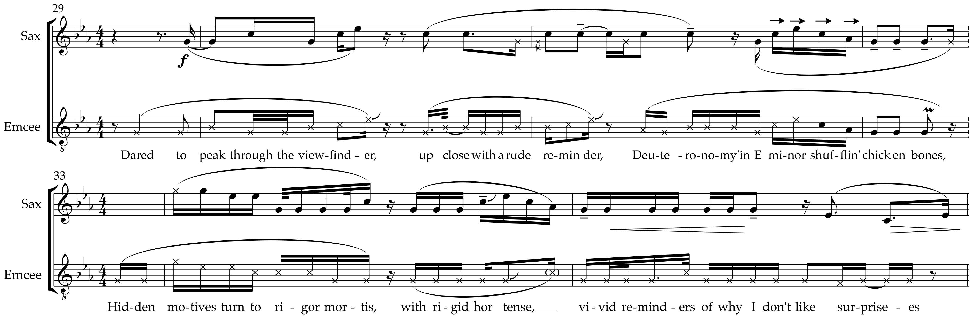
\includegraphics{images/figures/chp 03/120137nonciphermimesis.pdf}
        \caption{Mimesis in R.A.P. Ferreira's ``NONCIPHER,'' 1:20--1:37.}
        \label{fig:rorymimesis}
    \end{figure}
    \begin{itemize}
        \item Transcription of ``framing region'' and Verse 2, Vocal and Sax Lines
        \item Rory draws the ear to the saxophone work, live-tracked by Aaron shaw
        \item Demonstrating his own musical ear; showing that flow has a melodic dimension
    \end{itemize}
  
\phantomsection
\subsection*{\centering Moor Mother and billy woods (ft. Elucid)  -- ``Tiberius''}
\addcontentsline{toc}{subsection}{Moor Mother, billy woods, and Elucid's ``Tiberius''}

\begin{figure}[!p]
    \centering
    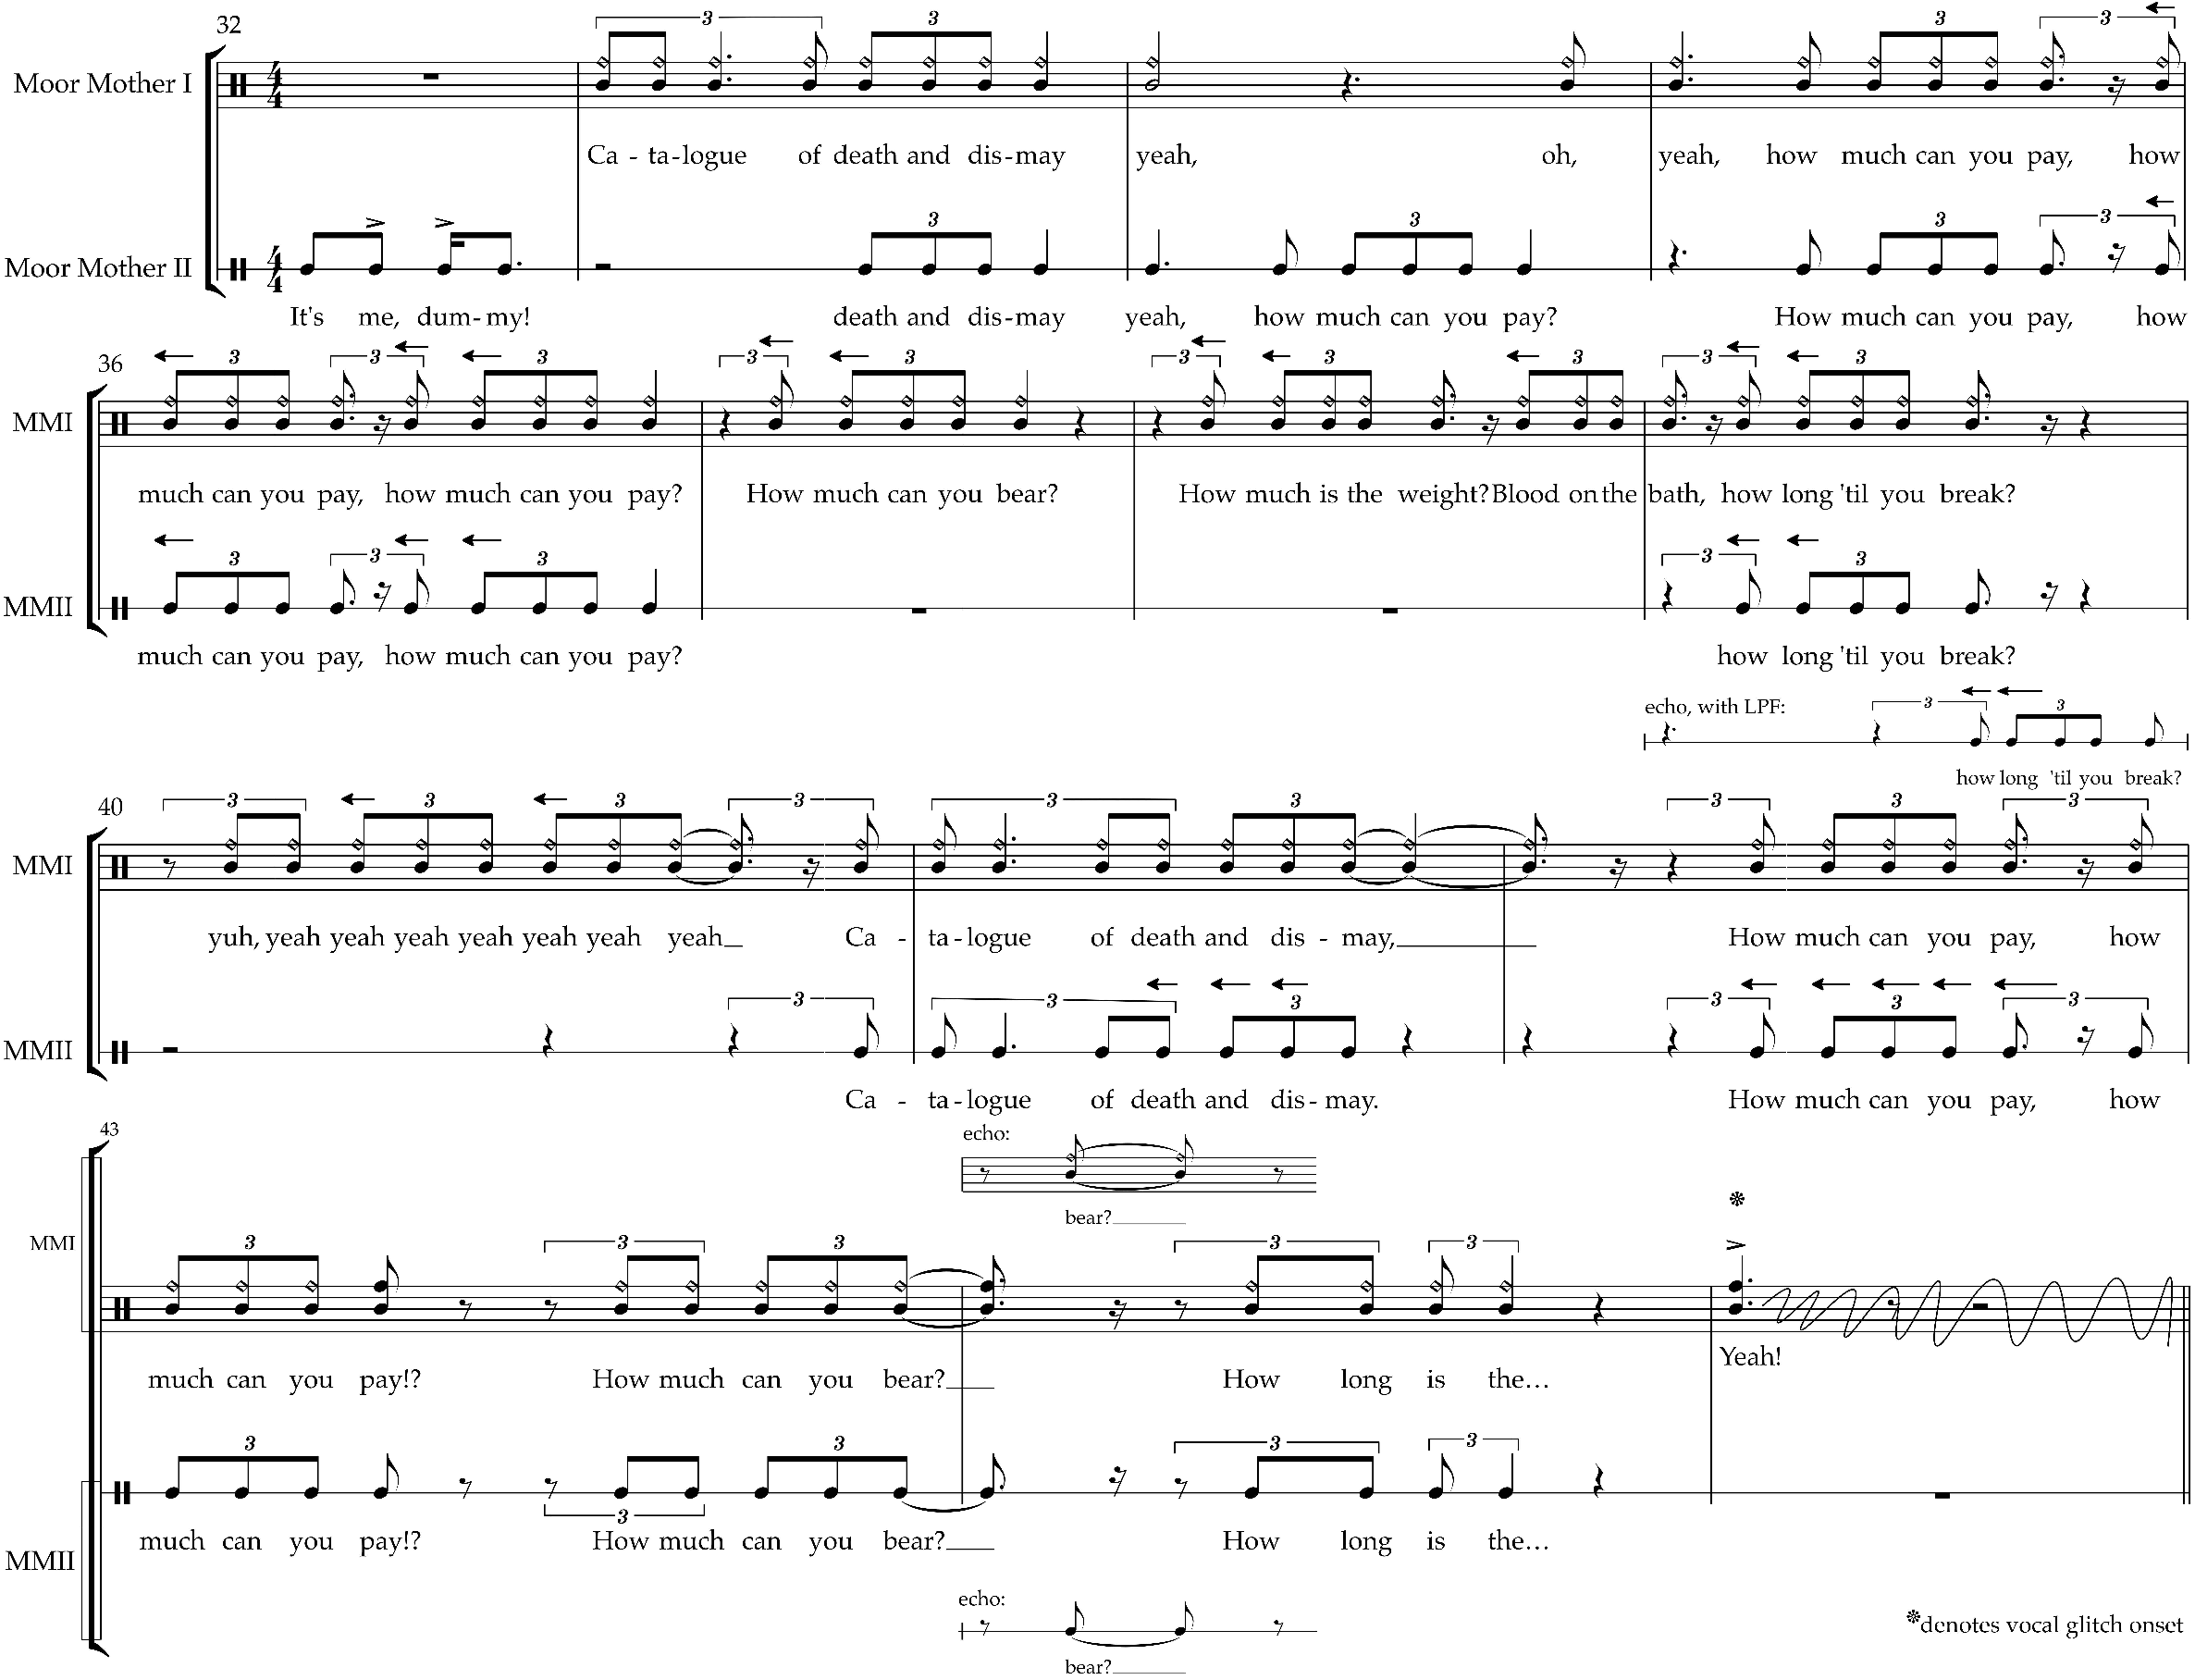
\includegraphics[width=\textwidth]{images/figures/chp 03/107136tiberiusprocessing.pdf}
    \caption{Vocal processing in Moor Mother and billy woods' ``Tiberius,'' 1:07--1:37.}
    \label{fig:moormotherprocess}
\end{figure}